\documentclass[aspectratio=169]{beamer}
\usepackage[utf8]{inputenc}
%\usepackage[authordate,backend=biber,natbib]{biblatex-chicago}
%\usepackage{booktabs}
%\addbibresource{growthreferences.bib}

%\usepackage{utopia} %font utopia imported

\usetheme{Madrid}
\usecolortheme{beaver}

%------------------------------------------------------------
%This block of code defines the information to appear in the
%Title page
\title[Diamond (2016)] %optional
{The Determinants and Welfare Implications of US Workers Diverging Location Choices by Skill: 1980-2000}

\subtitle{Rebecca Diamond, \emph{American Economic Review}, 2016}

\author [Hauk] % (optional)
{William~R.~Hauk,~Jr.} %\inst{1} %\and J.~Doe\inst{2}} 

\institute[UofSC] % (optional)
{
  %\inst{1}%
  Darla Moore School of Business\\
  University of South Carolina
  %\and
  %\inst{2}%
  %Faculty of Chemistry\\
  %Very Famous University
}

\date[ECON 860, Fall 2021] % (optional)
{ECON 860 -- International Trade Theory\\Fall 2021}

\logo{
\includegraphics[height=1cm]{UofSC_Monogram_Stack_CMYK_G.jpg}}

%End of title page configuration block

%---------------------------------------------------------

\AtBeginSection[]
{
  \begin{frame}
    \frametitle{Table of Contents}
    \tableofcontents[currentsection]
  \end{frame}
}

%------------------------------------------------------------

\begin{document}

%The next statement creates the title page.
\frame{\titlepage}

%-------------------------------------------------------------

\section{Introduction}

%-------------------------------------------------------------

\begin{frame}{Introduction}

Paper looks at two stylized facts:
\begin{itemize}
    \item<1-> Dramatic increase in the wage gap between high school and college graduates in the U.S. between 1980-2000.
    \item<2-> Some metropolitan areas receiving an increasing share of college graduates during 1980-2000.
    \item<3-> Creates phenomenon of the ``Great Divergence”.
\end{itemize}
    
\end{frame}

%-------------------------------------------------------------

\begin{frame}{Welfare Implications}

\begin{itemize}
    \item<1-> If college graduates have higher nominal wages, but live in more expensive cities, are they necessarily better off?
    \item<2-> Welfare implications might depend on the reason why there is this skill sorting.
    \item<3-> Changes in relative demand for high and low skill workers were a big driver of migration patterns.
    \item<4-> However, once cities attracted more college graduates, they became more desirable and expensive places to live.
    \item<5-> High-wage workers were willing to pay for amenities of large cities, low-wage workers were not.
\end{itemize}
    
\end{frame}

%-------------------------------------------------------------

\begin{frame}{Welfare Implications}

\begin{itemize}
    \item<1-> Overall impact is to increase the gap in well-being between college graduates and high school graduates over and above what would be indicated simply from wage inequality.
    \item<2-> As an example, Diamond looks at differing fates of Detroit and Boston.
    \begin{itemize}
        \item<3-> Detroit loses auto manufacturing jobs, but also suffers from declining educational attainment.
        \item<4-> Boston has attracted high-skill workers and has increasing educational attainment.
    \end{itemize}
\end{itemize}

\end{frame}

%-------------------------------------------------------------

\begin{frame}{Methodology}

\begin{itemize}
    \item<1-> Paper uses a structural spatial equilibrium model of cities in the spirit of Rosen (1979) and Roback (1982), but allows for workers to have heterogeneous preferences for cities.
    \item<2-> Workers with different characteristics make different trade-offs.  The most important worker characteristic is skill level – operationalized by graduation from a four-year college.
    \item<3-> A city’s skill-mix will influence local amenity levels – paper looks at 15 amenities, which is combined into a single index using Principal Component Analysis (PCA).
\end{itemize}
    
\end{frame}

%-------------------------------------------------------------

\begin{frame}{Estimation}

\begin{itemize}
    \item<1-> Workers’ preferences for cities are estimated using a two-step estimator.
    \begin{enumerate}
        \item<2-> First step, MLE is used to identify how desirable a city is to each type of worker.
        \item<3-> Second step is to use a simultaneous-equation, non-linear GMM estimator to estimate local labor demand, housing supply, labor supply, and amenity supply to cities.
    \end{enumerate}
    \item<4-> Model is identified using local labor demand shocks from the local industry mix and their interactions with local housing supply elasticities. 
\end{itemize}
    
\end{frame}

%-------------------------------------------------------------

\begin{frame}{Punchline}

\begin{itemize}
    \item<1-> While both college and noncollege workers find higher wages, lower rents, and higher amenity levels desirable, high skill workers’ demand is relatively more sensitive to amenity levels and low skill workers’ demand is more sensitive to wages and rents.
    \item<2->   Welfare impacts from wage, rent, and endogenous amenity changes led to an increase in well-being equivalent to at least a 25\% increase in the college wage gap – which is larger than the actual increase in the college wage gap.
\end{itemize}
    
\end{frame}

%-------------------------------------------------------------

\begin{frame}{Is This a Trade Paper?}

\begin{itemize}
    \item<1-> JEL Codes classify this primarily as a Labor Economics paper.
    \item<2-> However, results are important for the way that we think about the welfare effects of trade.
    \item<3-> Papers we have looked at thus far assume that trade shocks cause a reallocation of labor to more ``efficient” uses.  But what if the adjustment costs are non-trivial?
    \item<4-> Diamond establishes facts that Autor, Dorn, and Hanson will elaborate on next week – jobs created by trade are not always in the same places as jobs lost by trade.  Adjustment costs may be substantial.
\end{itemize}
    
\end{frame}

%-------------------------------------------------------------

\section{Data}

%-------------------------------------------------------------

\begin{frame}{Census IPUMS Data}

\begin{itemize}
    \item<1-> Paper uses the 5 percent samples of the US census from the 1980, 1990, and 2000 Integrated Public Use Microdata Series (IPUMS) dataset.
    \item<2-> All analysis is restricted to 25-55 year-olds working at least 35 hours per week and 48 weeks per year.
    \item<3-> The geographical unit of analysis is the metropolitan statistical area (MSA) of residence.  Census includes 218 MSAs across all three decades of data.  Rural areas are not in an MSA, but rural areas within each state are grouped together as a single MSA.
\end{itemize}
    
\end{frame}

%-------------------------------------------------------------

\begin{frame}{Education and Amenities}

\begin{itemize}
    \item<1-> Workers divided into college degree or higher and no four-year college degree, as this seems to be the biggest dividing line between skilled and nonskilled workers according to Katz and Murphy (1992) and Goldin and Katz (2008).
    \item<2-> Key variable is the local skill mix (ratio of college workers to noncollege workers) of workers in an MSA.
    \item<3-> MSA amenities classified into six categories – retail, transportation, crime, environmental, schooling, and job quality.
    \item<4-> MSA data supplemented with measures of geographic constraints and land use regulations to measure differences in housing supply elasticities.
\end{itemize}
    
\end{frame}

%-------------------------------------------------------------

\section{Descriptive Statistics}

%-------------------------------------------------------------

\begin{frame}{Summary Statistics}

\begin{figure}
    \centering
    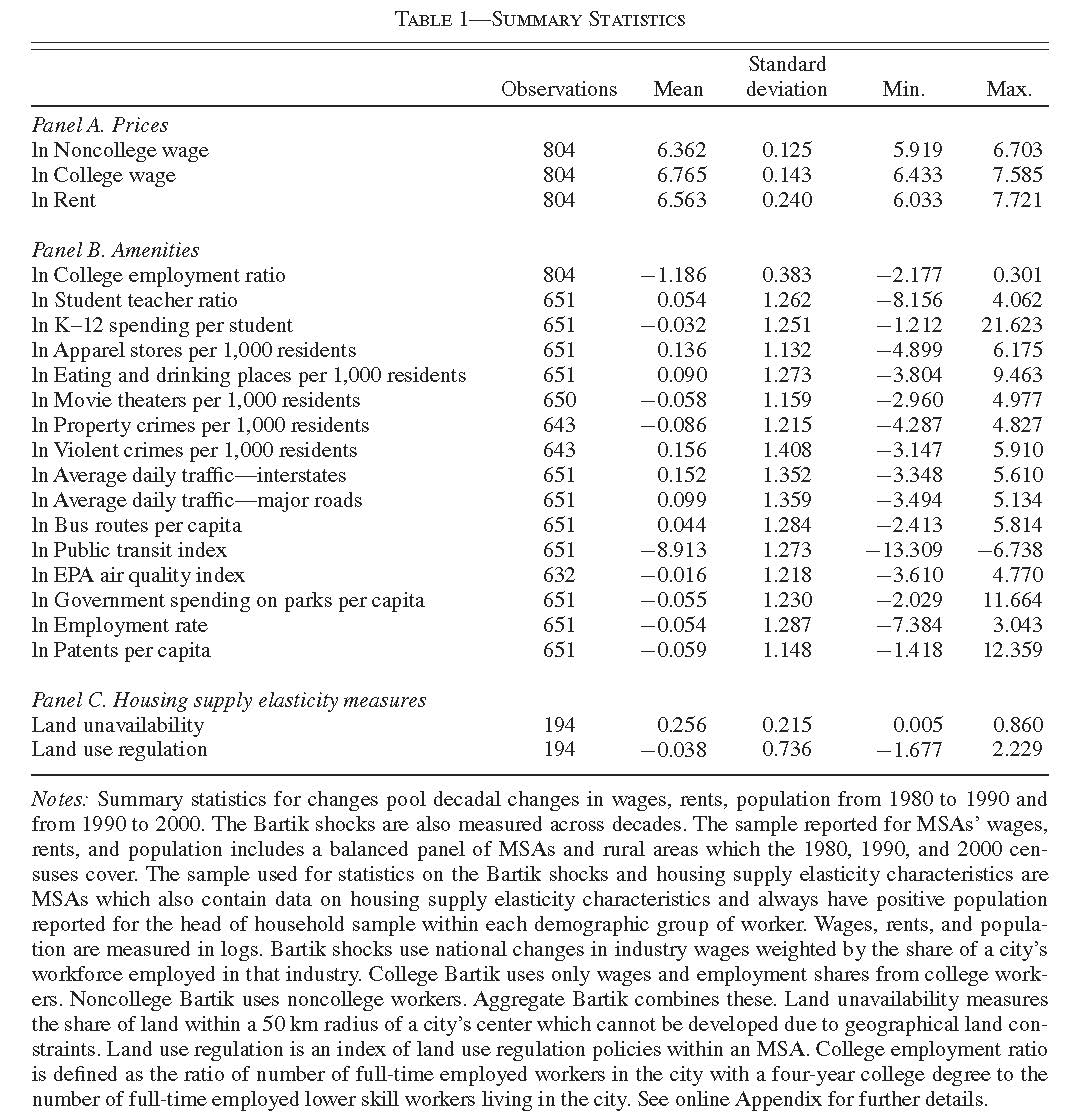
\includegraphics[scale=0.5]{DiamondTable1.jpg}
    \label{fig:Table1}
\end{figure}
    
\end{frame}

%-------------------------------------------------------------

\begin{frame}{Correlations}

\begin{figure}
    \centering
    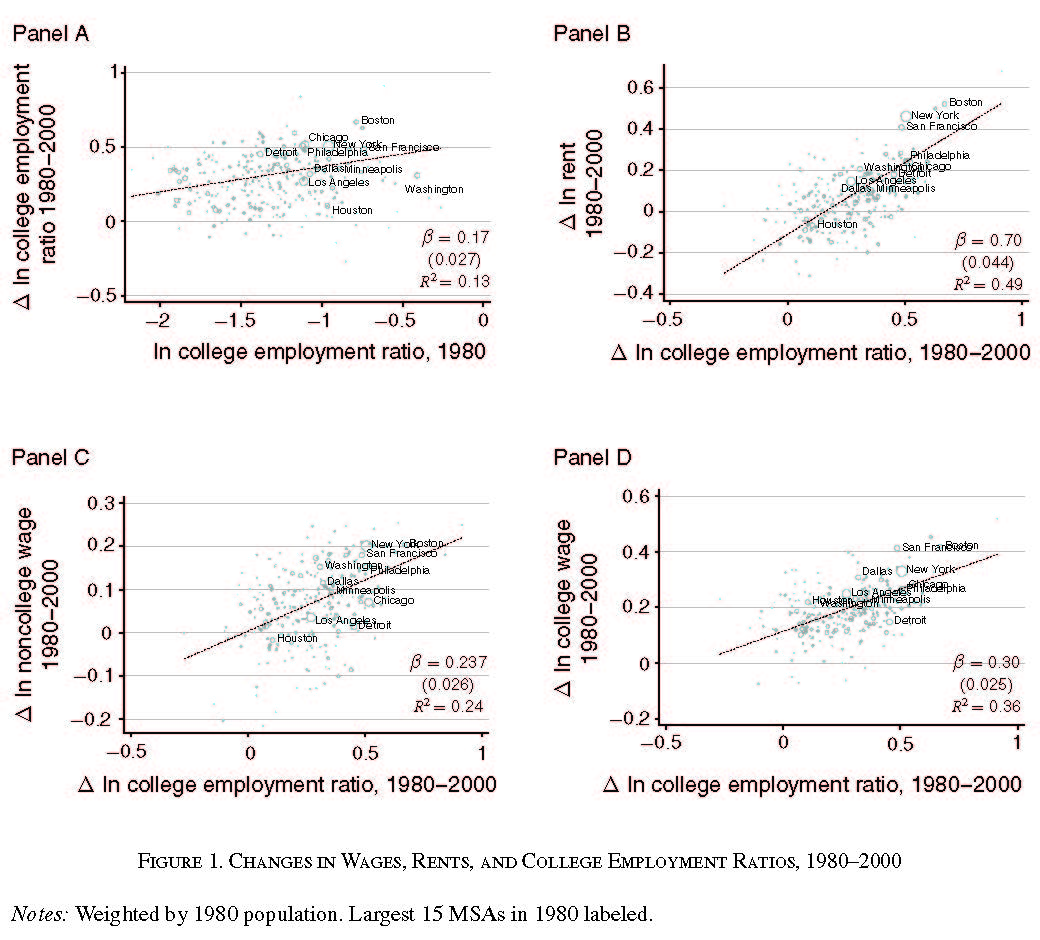
\includegraphics[scale=0.6]{DiamondFig1.jpg}
    \label{fig:Figure1}
\end{figure}
    
\end{frame}

%-------------------------------------------------------------

\begin{frame}{Correlations}

\begin{itemize}
    \item<1-> Panel A of Figure 1 shows that college employment ratio in 1980 is positively associated with growth in the college employment ratio from 1980-2000.  A 1\% increase in 1980 is associated with a 0.17\% larger increase from 1980-2000.
    \item<2-> Panel B of Figure 1 shows that an increase in the college employment ratio between 1980-2000 is positively associated with an increase in rents between 1980-2000.  A one percentage increase in college employment is associated with a 0.70\% increase in rents.
    \item<3-> Panel C of Figure 1 shows that an increase in the college employment ratio between 1980-2000 is positively associated with an increase in noncollege wages between 1980-2000.  A one percentage increase in college employment is associated with a 0.24\% increase in noncollege wages.
    \item<4-> Panel D of Figure 1 shows that an increase in the college employment ratio between 1980-2000 is positively associated with an increase in college wages between 1980-2000.  A one percentage in college employment is associated with a 0.30\% increase in college wages.
\end{itemize}
    
\end{frame}

%-------------------------------------------------------------

\begin{frame}{Wage Polarization}

The polarization of skill across cities coincided with a large nationwide increase in wage inequality.  Table 2 shows that the nationwide college/high school wage gap increased from 38\% in 1980 to 57\% in 2000.

\begin{figure}
    \centering
    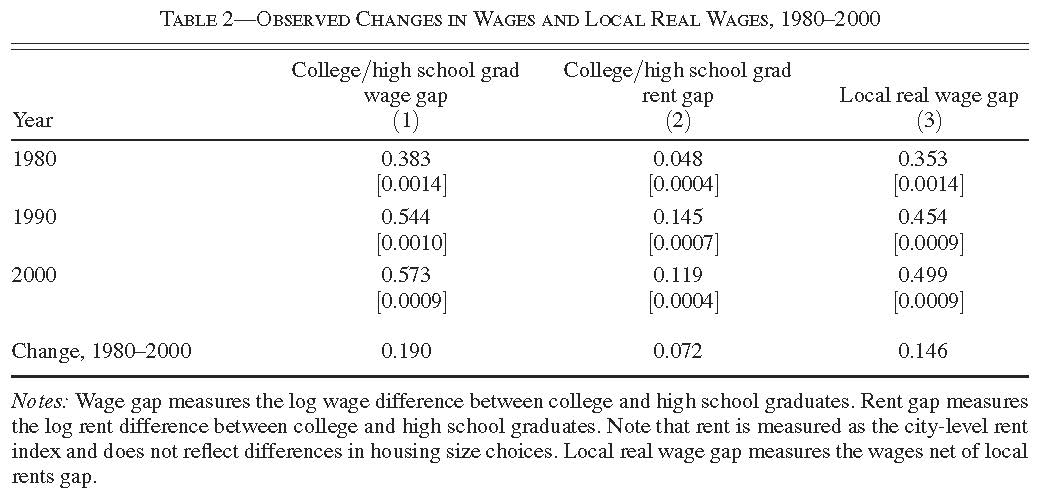
\includegraphics[scale=0.85]{DiamondTable2.jpg}
    \label{fig:Table2}
\end{figure}
    
\end{frame}

%-------------------------------------------------------------

\begin{frame}{Amenities Polarization}

Table 3 shows the relationships between changes in cities’ college employment ratios and their changes in a large set of local amenities.

\begin{figure}
    \centering
    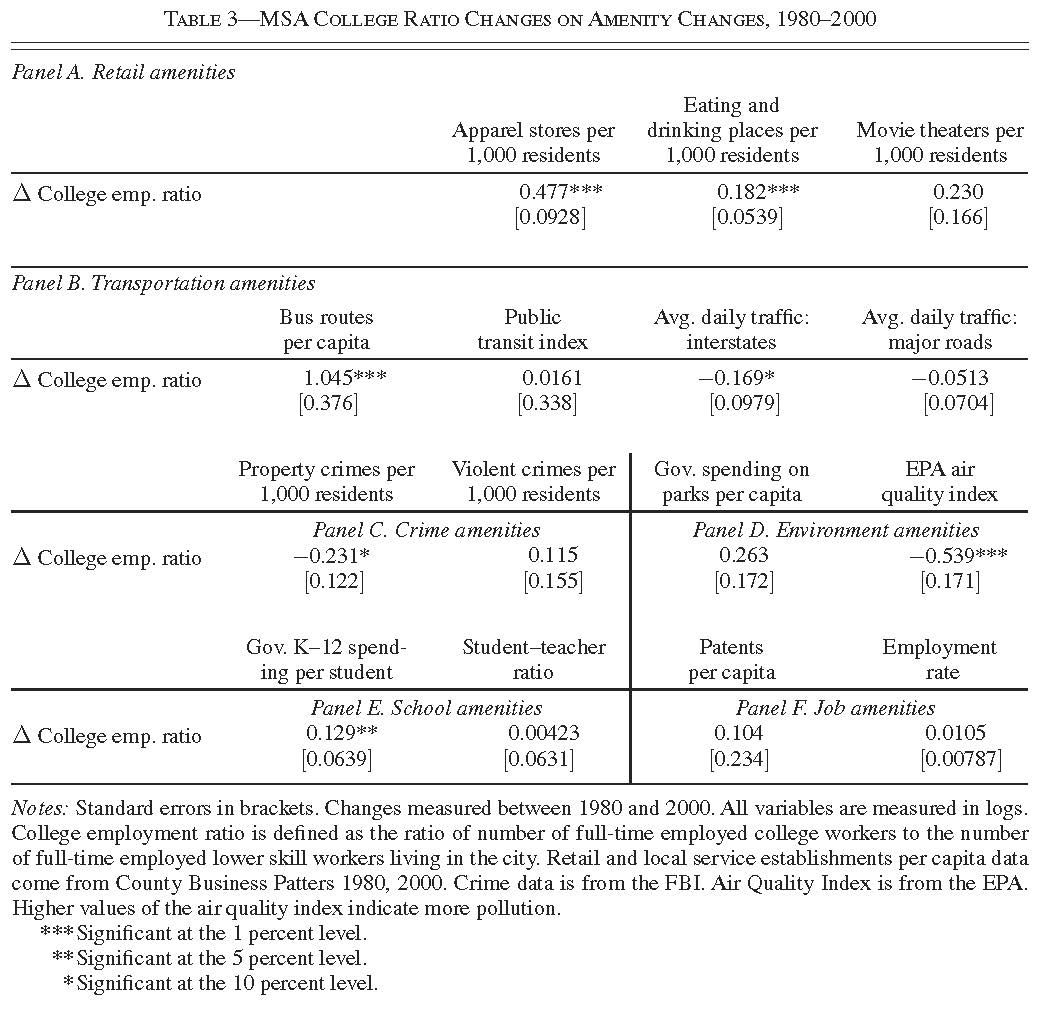
\includegraphics[scale=0.47]{DiamondTable3.jpg}
    \label{fig:Table3}
\end{figure}
    
\end{frame}

%-------------------------------------------------------------

\section{An Empirical Spatial Equilibrium Model of Cities}

%-------------------------------------------------------------

\begin{frame}{An Empirical Spatial Equilibrium Model of Cities}

\begin{itemize}
    \item<1-> In order to better understand how these observations affect welfare, one needs causal estimates of migration elasticities on these city characteristics.  Paper creates a structural model to estimate these elasticities.
    \item<2-> Structural model is similar to Rosen (1979) and Roback (1982), but allows more flexibility for heterogeneity in worker preferences and city housing supplies.
    \item<3-> Local worker productivity and amenities respond endogenously to the skill-mix of the city.
\end{itemize}
    
\end{frame}

%-------------------------------------------------------------

\subsection{Labor Demand}

%-------------------------------------------------------------

\begin{frame}{Labor Demand}

\begin{itemize}
    \item<1-> Each city $ j $ has many homogeneous firms $ d $ in year $ t $.
    \item<2-> These firms produce a homogeneous tradeable good using high skill labor $ H_{d,j,t} $, low skill labor $ L_{d,j,t} $, and capital $ K_{d,j,t} $ according to a Cobb-Douglas production function where high skill and low skill labor are substitutable:
    \begin{equation*}
        Y_{d,j,t} = N_{d,j,t}^{\alpha} K_{d,j,t}^{1 - \alpha}
    \end{equation*}
    where
    \begin{equation*}
        N_{d,j,t} = \left[ \theta_{j,t}^{L} L_{d,j,t}^{\rho} + \theta_{j,t}^{H} H_{d,j,t}^{\rho} \right]^{\frac{1}{\rho}}
    \end{equation*}
    and
    \begin{equation}
        \theta_{j,t}^{L} = f_{L}\left( H_{j,t}, L_{j,t} \right) \exp\left( e_{j,t}^L \right)
        \label{eq:lowskillproductivity}
    \end{equation}
    and
    \begin{equation}
        \theta_{j,t}^{H} = f_{H}\left( H_{j,t}, L_{j,t} \right) \exp\left( e_{j,t}^H \right)
        \label{eq:highskillproductivity}
    \end{equation}
\end{itemize}
    
\end{frame}

%-------------------------------------------------------------

\begin{frame}{Labor Productivity and Wages}

\begin{itemize}
    \item<1-> Equations (\ref{eq:lowskillproductivity}) and (\ref{eq:highskillproductivity}) show that labor productivity is determined by exogenous and endogenous factors.  Exogenous productivity shocks are given by the terms $ e_{j,t}^L $ and $ e_{j,t}^H $.
    \item<2-> While there is some evidence to indicate that the presence of more high skill workers leads to productivity spillovers for all workers, the functional form of the endogenous productivity functions $ f_L $ and $ f_H $ are agnostic for now.
    \item<3-> There are a large number of firms and no barriers to entry, so we can assume perfect competition and workers earn the value of their marginal product.  Capital is supplied elastically across all cities at price $ \kappa_t $. So:
    \begin{equation*}
        \begin{split}
            W_{j,t}^{H} &= \alpha N_{d,j,t}^{\alpha - \rho} K_{d,j,t}^{1 - \alpha} H_{d,j,t}^{\rho - 1} f_{H}\left( H_{j,t}, L_{j,t} \right) \exp\left( \varepsilon_{j,t}^{H} \right) \\
            W_{j,t}^{L} &= \alpha N_{d,j,t}^{\alpha - \rho} K_{d,j,t}^{1 - \alpha} L_{d,j,t}^{\rho - 1} f_{L}\left( H_{j,t}, L_{j,t} \right) \exp\left( \varepsilon_{j,t}^{L} \right) \\
            \kappa_{t} &= N_{d,j,t}^{\alpha} K_{d,j,t}^{-\alpha}\left( 1 - \alpha \right)
        \end{split}
    \end{equation*}
\end{itemize}
    
\end{frame}

%-------------------------------------------------------------

\begin{frame}{Aggregate Labor Demand}

Firm level labor demand translates directly into city-level aggregate labor demand as firms within a city all have an identical constant-returns-to-scale production technology:

\begin{equation*}
    \begin{split}
        w_{j,t}^{H} &= \log\left( W_{j,t}^H \right) = c_{t} + \left( 1 - \rho \right) \ log\left( N_{j,t} \right) + \left( \rho - 1 \right) \log \left( H_{j,t} \right) + \log\left( f_{H}\left( H_{j,t}, L_{j,t} \right) \right) + \varepsilon_{j,t}^{H} \\
        w_{j,t}^{L} &= \log\left( W_{j,t}^L \right) = c_{t} + \left( 1 - \rho \right) \ log\left( N_{j,t} \right) + \left( \rho - 1 \right) \log \left( L_{j,t} \right) + \log\left( f_{L}\left( H_{j,t}, L_{j,t} \right) \right) + \varepsilon_{j,t}^{L} \\
        N_{j,t} &= \left( \exp\left( \varepsilon_{j,t}^{L} \right) f_{L}\left( H_{j,t}, L_{j,t} \right) L_{j,t}^{\rho} + \exp\left( \varepsilon_{j,t}^{H} \right) f_{H}\left( H_{j,t}, L_{j,t} \right) H_{j,t}^{\rho} \right)^{\frac{1}{\rho}}
    \end{split}
\end{equation*}
where:
\begin{equation*}
    c_{t} = \log\left( \alpha \left( \frac{1 - \alpha}{\kappa_{t}} \right)^{\frac{1 - \alpha}{\alpha}} \right)
\end{equation*}
    
\end{frame}

%-------------------------------------------------------------

\begin{frame}{Aggregate Labor Demand}

\begin{itemize}
    \item<1-> Labor supply impacts wages through two channels: imperfect labor substitution of high and low skill workers within firms (governed by $ \rho $) and city wide productivity changes (governed by $ f_H $ and $ f_L $).
    \item<2-> Instead of imposing parametric restrictions, the labor demand functions can be rewritten as: \begin{equation*}
        \begin{split}
            w_{j,t}^{H} &= g_{H}\left( H_{j,t}, L_{j,t} \right) + \varepsilon_{j,t}^{H} \\
            w_{j,t}^{L} &= g_{L}\left( H_{j,t}, L_{j,t} \right) + \varepsilon_{j,t}^{L}
        \end{split}
    \end{equation*}
    \item<2-> We can approximate these functions using a log-linear specification:
    \begin{equation*}
        w_{j,t}^{H} = \gamma_{HH} \log{H_{j,t}} + \gamma_{HL} \log{L_{j,t}} + \varepsilon_{j,t}^{H}
    \end{equation*}
    and
    \begin{equation*}
        w_{j,t}^{L} = \gamma_{LH} \log{H_{j,t}} + \gamma_{LL} \log{L_{j,t}} + \varepsilon_{j,t}^{L}
    \end{equation*}
\end{itemize}
    
\end{frame}

%-------------------------------------------------------------

\subsection{Labor Supply to Cities}

%-------------------------------------------------------------

\begin{frame}{Labor Supply}

\begin{itemize}
    \item<1-> Each head-of-household worker $ i $ chooses to live in the city that offers him or her the most desirable bundle of wages, local good prices, and amenities, where wages are determined by the worker's education level.
    \item<2-> The worker consumes a local good $ M $, which has a local price $ R_{j,t} $, and a national good $ O $, which has a national price $ p_{t} $, and gains utility from the vector of amenities $ A_{j,t} $ in the city.
    \item<3-> The worker has Cobb-Douglas preferences for the local and national good, and the utility function looks like:
    \begin{equation*}
        \max_{M,O} \log\left( M^{\xi} \right) + \log\left( O^{1 - \xi} \right) + s_{i}\left( A_{j,t} \right)
    \end{equation*}
    subject to:
    \begin{equation*}
        P_{t} O + R_{j,t} M \le W_{j,t}^{edu}
    \end{equation*}
\end{itemize}
    
\end{frame}

%-------------------------------------------------------------

\begin{frame}{Worker's Utility}

\begin{itemize}
    \item<1-> The worker’s optimized utility function can be expressed as an indirect utility function
    \begin{equation*}
        V_{i,j,t} = \log\left( \frac{w_{j,t}^{edu}}{P_{t}} \right) - \xi \log\left( \frac{R_{j,t}}{P_{t}} \right) + s_{i} \left( A_{j,t} \right)
    \end{equation*}
    or
    \begin{equation}
        V_{i,j,t} = w_{j,t}^{edu} - \xi r_{j,t} + s_{i} \left( A_{j,t} \right)
        \label{eq:indirectutility1}
    \end{equation}
    \item<2-> The price index used in the denominator above, is the CPI-U index for all goods excluding shelter measured in year 2000 U.S. dollars.
    \item<3-> The workers’ optimized utility function also leads to his local good demand
    \begin{equation*}
        HD_{i,j,t} = \frac{\xi w_{j,t}^{edu}}{R_{j,t}}
    \end{equation*}
\end{itemize}
    
\end{frame}

%-------------------------------------------------------------

\begin{frame}{Amenities and Labor Supply}

\begin{itemize}
    \item<1-> Some amenities are exogenous to the labor market mix of the city – define this as vector $ x_{j,t}^{A} $. Other amenities respond endogenously to the labor mix. Specifically, define $ a_{j,t} $ as the first principal comoponent of a bundle of amenities related to school quality, retail, crime, the environment, transportation, and the quality of the job market.
    \item<2-> The function $ s\left( A_{j,t} \right) $ maps the vector of city amenities to the worker's utility value for them:
    \begin{equation*}
        \begin{split}
            s\left( A_{j,t} \right) &= a_{j,t} \beta_{i}^{a} + x_{j,t}^{A} \beta_{i}^{x} + \beta_{i}^{st} x_{j}^{st} + \beta_{i}^{div} x_{j}^{div} + \sigma_{i} \varepsilon_{i,j,t} \\
            \beta_{i}^{x} &= \beta^{x} z_{i} \\
            \beta_{i}^{a} &= \beta^{a} z_{i} \\
            \beta_{i}^{st} &= st_{i} \beta^{st} z_{i} \\
            \beta_{i}^{div} &= div_{i} \beta^{div} z_{i} \\
            \sigma_{i} &= \beta^{\sigma} z_{i} \\
            \varepsilon_{i,j,t} &\sim \text{Type I Extreme Value}
        \end{split}
    \end{equation*}
\end{itemize}
    
\end{frame}

%-------------------------------------------------------------

\begin{frame}{Amenities and Labor Supply}

\begin{itemize}
    \item<1-> $ \beta_{i}^{st} $ and $ \beta_{i}^{div} $ measure a worker's value of living in his or her state of birth and census division of birth.
    \item<2-> Worker $ i $'s marginal utility of the different types of amenities are a function of a $ 3 \time 1 $ vector of demographic variables $ z_{i} $, which include dummy variables indicating if a worker is white, black, or an immigrant.
    \item<3-> $ x_{j}^{st} $ is a $ 50 \times 1 $ vector where each element $ k $ takes on a value of 1 if MSA $ j $ is partly located in state $ k $.  Similarly, $ x_{j}^{div} $ is a $ 9 \times 1 $ vector where element $ k $ takes on a value of 1 if MSA $ j $ is located in census division $ k $.
\end{itemize}
    
\end{frame}

%-------------------------------------------------------------

\begin{frame}{Utility Function Revisited}

\begin{itemize}
    \item<1-> $ \varepsilon_{i,j,t} $ is an idiosyncratic preference term for worker $ i $.  The indirect utility function (\ref{eq:indirectutility1}) is renormalized by dividing each worker’s utility by $ \beta^{\sigma} z_{i} $ so that the standard deviation of worker idiosyncratic preferences is normalized to 1.
    \item<2-> The indirect utility function for worker $ i $ in city $ j $ can now be written as:
    \begin{equation*}
        V_{i,j,t} = \left( w_{j,t}^{edu} - \xi r_{j,t} \right) \beta^{w} z_{i} + a_{j,t} \beta_{i}^{a} + x_{j,t} \beta_{i}^{x} + x_{j}^{st}\beta_{i}^{st} + x_{j}^{div} \beta_{i}^{div} + \varepsilon_{i,j,t}
    \end{equation*}
    \item<3-> Define $ \delta_{j,t}^{z} $ as the utility value of the components of city $ j $ that all workers of type $ z $ value identically:
    \begin{equation*}
        \delta_{j,t}^{z} = \left( w_{j,t}^{edu} - \xi r_{j,t} \right) \beta^{w} z_{i} + a_{j,t} \beta_{i}^{a} z_{i} + x_{j,t} \beta_{i}^{x} z_{i}
    \end{equation*}
    and rewriting the utility function in terms of $ \delta_{j,t}^{z} $, we have:
    \begin{equation*}
        V_{i,j,t} = \delta_{j,t}^{z} + x_{j}^{st}\beta_{i}^{st} z_{i} + x_{j}^{div} \beta_{i}^{div} z_{i} + \varepsilon_{i,j,t}
    \end{equation*}
\end{itemize}
    
\end{frame}

%-------------------------------------------------------------

\begin{frame}{Conditional Logit Model}

\begin{itemize}
    \item<1-> The total expected population of city j is simply the probability that each worker lives in the city, summed over all workers.  This can be rewritten as a conditional logit model for high skill workers:
    \begin{equation*}
        H_{j,t} = \sum_{i \in H_{t}} \frac{\exp\left( \delta_{j,t}^{z} + x_{j}^{st}\beta_{i}^{st} z_{i} + x_{j}^{div} \beta_{i}^{div} z_{i} \right)}{\sum_{k}^{J} \exp\left( \delta_{j,t}^{z} + x_{j}^{st}\beta_{i}^{st} z_{i} + x_{j}^{div} \beta_{i}^{div} z_{i} \right)}
    \end{equation*}
    and for low skill workers:
    \begin{equation*}
        L_{j,t} = \sum_{i \in L_{t}} \frac{\exp\left( \delta_{j,t}^{z} + x_{j}^{st}\beta_{i}^{st} z_{i} + x_{j}^{div} \beta_{i}^{div} z_{i} \right)}{\sum_{k}^{J} \exp\left( \delta_{j,t}^{z} + x_{j}^{st}\beta_{i}^{st} z_{i} + x_{j}^{div} \beta_{i}^{div} z_{i} \right)}
    \end{equation*}
    \item<2->Observed variables are the high and low skilled population, wages, rent, the amenity index, worker demographics, and workers’ states and census divisions of birth.  Exogenous amenities and idiosyncratic taste preferences are unobserved.  Estimated parameters are the workers’ preferences for wages, rent, and amenities ($ \beta $, $ \xi $).
\end{itemize}
    
\end{frame}

%-------------------------------------------------------------

\end{document}